\documentclass[conference]{IEEEtran}
\IEEEoverridecommandlockouts

\usepackage{cite}
\usepackage{amsmath,amssymb,amsfonts}
\usepackage{graphicx}
\usepackage{textcomp}
\usepackage{xcolor}
\usepackage{booktabs}
\usepackage{multirow}
\usepackage{microtype}

\begin{document}

\title{MIS: Diagnosing Structural Bottlenecks in Copy-Paste Augmentation
for Agricultural Object Detection}

\author{
    \IEEEauthorblockN{Huy Khanh Tran, Yuichiro Nomura, and Hiroshi Mineno}
    \IEEEauthorblockA{Graduate School of Integrated Science and Technology,
    Shizuoka University, Japan \\
    tran.huy.khanh.25@shizuoka.ac.jp}
}

\maketitle

\begin{abstract}
Copy-paste augmentation achieves strong results for instance
segmentation yet yields inconsistent or negative gains for
bounding-box detection in agricultural scenes.
We propose the \textbf{Minimum Inference Score (MIS)}, a difficulty
metric derived from a trained baseline detector that correlates with
detection failure modes---miss rate and false-positive rate---across
objects and images.
MIS reveals where a model fails in a dataset: when MIS detects strong or 
moderate concentration of hard instances
in near-zero AP regimes---regardless of whether the structural source
is object size, domain composition, or both---copy-paste augmentation
cannot provide reliable gains.
We demonstrate this as a pre-augmentation diagnostic validated
across three agricultural benchmarks, where MIS correctly anticipates
failure under structural constraints and consistent gains in their absence.
\end{abstract}

\begin{IEEEkeywords}
object detection, copy-paste augmentation, difficulty scoring,
agricultural object detection, data augmentation diagnostic
\end{IEEEkeywords}

% ----------------------------------------------------------
\section{Introduction}

Copy-paste augmentation composites cropped labeled instances into
training images to increase sampling diversity~\cite{kisantal2019augmentation,
ghiasi2021simple}.
While effective for instance
segmentation~\cite{ghiasi2021simple}, bounding-box detection in
agricultural imagery is subject to harsher constraints---sub-resolution
instances, multi-domain acquisition, and high object
density---frequently producing inconsistent or negative augmentation
outcomes and forcing costly multi-seed search without a principled
stopping criterion.

We introduce the \textbf{Minimum Inference Score (MIS)}, a
metric computed from a trained baseline detector that captures
model failure patterns on a given dataset.
By correlating with miss rate and FP rate, MIS surfaces where difficulty
concentrates in a dataset (driven by object size, domain composition or their interaction) 
and helps determine whether copy-paste can provide
useful training signal. 
On MinneApple~\cite{hani2020minneapple},
GWHD~2021~\cite{david2021global}, and
WGISD~\cite{santos2020grape}, MIS correctly anticipates failure when
hard instances concentrate in structurally constrained regimes and
consistent gains when no such constraint is present,
providing bidirectional diagnostic validation.

% ----------------------------------------------------------
\section{Methodology}
\subsection{Scoring Formulation}

Let $G(I)$ denote ground-truth boxes in image $I$.
A trained detector produces predictions $p$ with confidence $c_p$ at
$\tau_{\mathrm{conf}}{=}0.001$ to retain near-miss candidates.
For each $g\in G(I)$, let
$\mathcal{P}(g){=}\{p:\mathrm{IoU}(p,g){\ge}0.5\}$.
The \textit{Object Difficulty Score} is
\begin{equation}
S_{\mathrm{obj}}(g) =
\begin{cases}
  \min_{p \in \mathcal{P}(g)}\!
    [\alpha(1{-}c_p) + \beta(1{-}u_p)],
    & \mathcal{P}(g) \neq \varnothing \\[2pt]
  \alpha + \beta, & \mathcal{P}(g) = \varnothing
\end{cases}
\label{eq:obj}
\end{equation}
with $\alpha{=}\beta{=}0.5$ and $u_p{=}\mathrm{IoU}(p,g)$.
Unmatched objects receive the maximum score $(\alpha{+}\beta{=}1)$.
The \textit{Image Difficulty Score} is
\begin{equation}
S_{\mathrm{img}}(I)
  = \frac{1}{|G(I)|}\sum_{g} S_{\mathrm{obj}}(g)
  + w_2 \cdot \mathrm{FPrate}(I),
\label{eq:img}
\end{equation}
where $\mathrm{FPrate}(I)$ counts unmatched predictions per image.
This yields $S_{\mathrm{obj}} \in [0,1]$ for every ground-truth object
and $S_{\mathrm{img}}$ for every training image, where higher values
indicate greater detection difficulty.
By construction, $S_{\mathrm{img}}$ encodes both axes of detection
failure (miss rate and FP rate); $w_2$ is set by grid search to
balance their contributions.

\subsection{Augmentation Protocol}
We train a YOLOv8s baseline and partition all training objects by
$S_{\mathrm{obj}}$ and all training images by $S_{\mathrm{img}}$ into
equal difficulty tertiles (Low, Medium, High).
Four copy-paste conditions are evaluated:
\textbf{Score High} pastes objects from the highest-difficulty object
tertile into the highest-difficulty destination images;
\textbf{Score Medium} and \textbf{Score Low} follow the same logic
for their respective tertiles.
\textbf{Random} selects both destination images and source objects
without score-based filtering.
This design isolates whether directing augmentation toward specific
difficulty regimes affects outcome.
Following~\cite{kisantal2019augmentation}, training data is expanded
by 30\% via unblended within-image copy-paste: 2--8 objects per
image, scale~$[0.9,1.1]$, rotation~$\pm15^\circ$,
$3{\times}$~maximum reuse; all other settings follow the default
YOLOv8 protocol.


% ----------------------------------------------------------
\section{Results}
\subsection{MIS Reflects Detection Failure Modes}

Pearson correlations between $S_{\mathrm{img}}$ and miss rate are
$r{=}0.66$, $0.75$, $0.63$ on MinneApple, GWHD, and WGISD;
correlations with FP rate are $r{=}0.63$, $0.75$, $0.64$.
Consistent moderate-to-strong correlations across all three datasets
confirm that MIS captures the primary axes of detection failure as
intended by its construction.

\subsection{MIS Identifies Structural Failure Sources}

\textbf{Size (MinneApple).}
$S_{\mathrm{obj}}$ inversely tracks AP across size groups
(Spearman~$r_s{=}{-}0.82$; Table~\ref{tab:size_val}):
64.4\% of the top-difficulty tertile falls in \textit{Very Small}
instances (${\le}400$\,px$^2$), where AP is near-zero ($0.071$),
indicating hard objects concentrate below the model's size recognition
threshold.

\textbf{Domain (GWHD~2021).}
Per-domain median MIS strongly anticorrelates with domain AP
(Pearson~$r{=}{-}0.90$; Fig.~\ref{fig:gwhd}): MIS correctly
ranks domain difficulty from detector behavior alone,
regardless of its underlying cause---varied cameras,
growth stages, and geographic acquisition conditions.


\begin{table}[t]
\centering
\caption{MinneApple: $S_{\mathrm{obj}}$ captures size-level difficulty.}
\label{tab:size_val}
\footnotesize
\setlength{\tabcolsep}{3.5pt}
\renewcommand{\arraystretch}{0.95}
\begin{tabular}{lccc}
\toprule
\textbf{Category} & \textbf{AP} & \textbf{Mean $S_{\mathrm{obj}}$}
  & \textbf{Top tertile} \\
\midrule
Very Small ($\le$400\,px$^2$) & 0.071 & 0.152 & 64.4\% \\
Small (400--1024\,px$^2$)     & 0.270 & 0.076 & 33.9\% \\
Medium ($>$1024\,px$^2$)      & 0.493 & 0.053 &  1.7\% \\
\bottomrule
\end{tabular}
\end{table}

\begin{figure}[t]
  \centering
  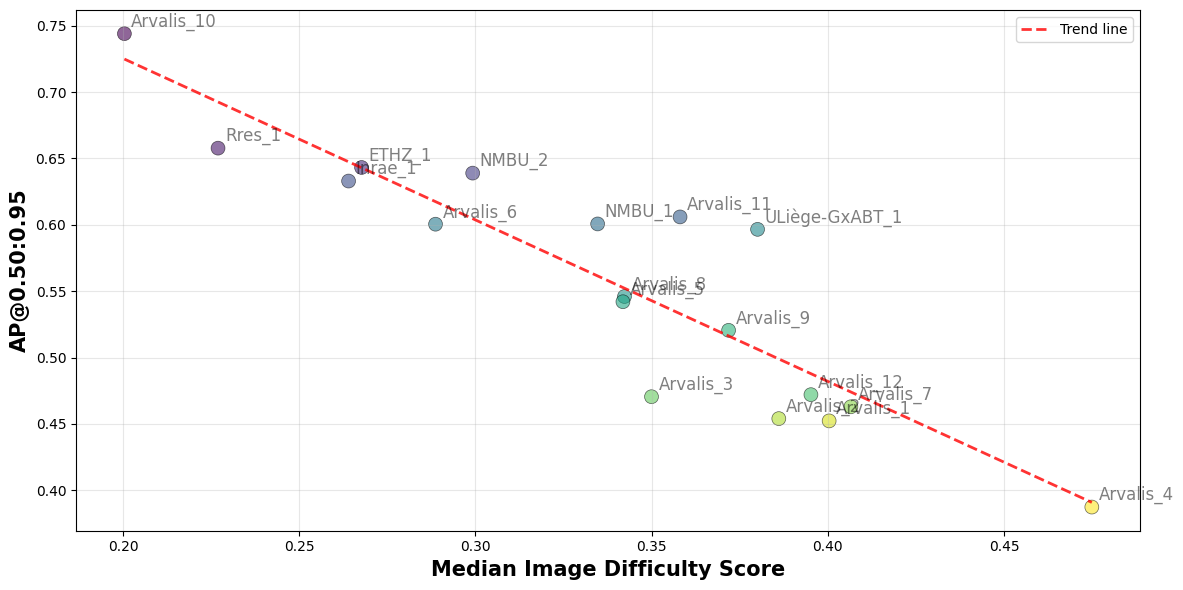
\includegraphics[width=\columnwidth]{gwhd_domain_score.png}
  \caption{GWHD~2021: per-domain AP vs.\ median image difficulty (MIS).}
  \label{fig:gwhd}
\end{figure}

\subsection{Application: Pre-Augmentation Diagnostic for Copy-Paste}

\textbf{MinneApple (resolution ceiling).}
MIS identifies hard objects concentrated below the recognition
threshold.
All four copy-paste conditions yield negative AP
(Table~\ref{tab:outcomes}), confirming that
additional sub-resolution instances provide no usable
learning signal regardless of selection strategy.

\textbf{GWHD~2021 (domain difficulty).}
MIS partitioning reveals near-complete domain separation:
low-difficulty images are 66\% in ETHZ\_1/Rres\_1 domain with
(AP\,${\approx}$\,0.70), while high-difficulty images are
78\% Arvalis variants (AP\,${\approx}$\,0.40--0.47).
This structure directly predicts per-condition behavior.
Score~Low sources from high-AP domains, reinforcing
already well-learned patterns which result in consistent, low-variance
drop ($-0.034$, $\sigma{=}0.005$).
Score~High sources from hard Arvalis domains where
difficulty is acquisition-based; added instances cannot
resolve domain gaps, yielding high instability
($-0.006$, $\sigma{=}0.040$).
Random and Medium sample without domain awareness,
producing moderate drops ($-0.015$, $-0.017$) at
intermediate variance ($\sigma{=}0.023$, $0.021$).
Outcome variance scales monotonically with
sourced-domain difficulty---a pattern that we can use MIS 
to predicts
from partition composition alone, before any augmented run.

\textbf{WGISD (positive control).}
MIS flags no structural bottleneck: unlike MinneApple
and GWHD, $S_{\mathrm{obj}}$ shows no dominant
concentration in near-zero AP size or domain regimes,
and baseline AP is non-negligible across all object groups.
All conditions yield positive gains (Table~\ref{tab:outcomes}), 
with Score~Medium achieving
the best result, confirming copy-paste viability
when MIS raises no flag.

Across all three benchmarks, the \emph{direction} of
copy-paste outcome is consistent with the MIS diagnostic:
all conditions are negative on flagged datasets and
positive on the unflagged dataset.
This directional consistency, independent of selection
strategy, supports a structural rather than
selection-driven explanation and directly addresses
why copy-paste struggles: it cannot overcome the
underlying difficulty MIS identifies.

\begin{table}[t]
\centering
\caption{Copy-paste outcomes (3-seed mean $\pm\,\sigma$).
Bottleneck: structural failure source identified by MIS.}
\label{tab:outcomes}
\footnotesize
\setlength{\tabcolsep}{2.5pt}
\renewcommand{\arraystretch}{0.95}
\begin{tabular}{lllll}
\toprule
\textbf{Dataset}
  & \textbf{Bottleneck}
  & \textbf{Base AP}
  & \textbf{Best $\Delta$}
  & \textbf{Worst $\Delta$} \\
\midrule
MinneApple
  & Size
  & $0.353\pm0.005$
  & $-0.003$ (Hi)
  & $-0.008$ (Rnd) \\
GWHD~2021
  & Domain
  & $0.229\pm0.013$
  & $-0.006^{*}$ (Hi)
  & $-0.034$ (Lo) \\
WGISD
  & ---
  & $0.480\pm0.007$
  & $+0.009$ (Med)
  & $+0.001$ (Hi) \\
\bottomrule
\multicolumn{5}{l}{\scriptsize
  $^*$Score High on GWHD: $\sigma{=}0.040$, high seed variance.}
\end{tabular}
\end{table}


% ----------------------------------------------------------
\section{Conclusion}

MIS links baseline detector failure behavior to difficulty 
concentration patterns, enabling a 
practical pre-augmentation signal that indicates whether 
copy-paste is likely to yield reliable gains.
In our experiments, 24 augmented training runs across MIS-flagged
datasets (MinneApple and GWHD, 4 conditions $\times$ 3 seeds each)
yielded zero reliable gains; MIS identifies these datasets without
any augmented run, directly saving that compute budget.
Practitioners should apply MIS after baseline training:
when MIS identifies strong or moderate concentration of 
high-difficulty instances in near-zero AP regimes, copy-paste augmentation 
is unlikely to yield reliable gains.
This finding is validated bidirectionally across three agricultural
benchmarks.
Future work includes using MIS to guide instance-level selection
when structural constraints are absent, and combining MIS with
generative methods to produce information-rich training instances
for hard regimes.

\section*{Acknowledgment}
This work was supported by JST FOREST JPMJFR201B,
JSPS KAKENHI JP25H01110.

\begin{thebibliography}{00}

\bibitem{kisantal2019augmentation}
M.~Kisantal \textit{et~al.},
``Augmentation for small object detection,''
\textit{arXiv:1902.07296}, 2019.

\bibitem{ghiasi2021simple}
G.~Ghiasi \textit{et~al.},
``Simple copy-paste is a strong data augmentation method for
instance segmentation,''
in \textit{Proc.\ CVPR}, 2021, pp.~2918--2928.

\bibitem{hani2020minneapple}
N.~H\"{a}ni, P.~Roy, and V.~Isler,
``MinneApple: A benchmark dataset for apple detection and
segmentation,''
\textit{IEEE RA-L}, vol.~5, no.~2, pp.~852--858, 2020.

\bibitem{david2021global}
E.~David \textit{et~al.},
``Global wheat head detection 2021,''
\textit{Plant Phenomics}, 2021.

\bibitem{santos2020grape}
T.~T.~Santos \textit{et~al.},
``Grape detection, segmentation, and tracking using deep
neural networks,''
\textit{Comput.\ Electron.\ Agric.}, vol.~170, p.~105247, 2020.

\end{thebibliography}

\end{document}